\section{What the cash becomes separates the trajectories}
\label{sec:conversion}

\subsection{Sellers: paying for houses or postponing insolvency}

A sale that completes a rival's group can serve two purposes. It can raise cash to survive, or it can pay for houses on the seller's own group. We split the \fact{barg.dyads.settled-one-sided} one-sided sales by whether the seller bought at least one house or hotel within eight turns of the sale, which is two rounds of a full table (Table~\ref{tab:sellers}).

\begin{table}[t]
\centering\small
\begin{tabular}{@{}llrrrr@{}}
\toprule
& & & Seller & Seller later & Median turns\\
Seller's cash at the sale & After the sale the seller & Sales & won & eliminated & to elimination\\
\midrule
\SellerRows
\bottomrule
\end{tabular}
\caption{What followed the \fact{barg.dyads.settled-one-sided} sales that completed a color group for the buyer only. A seller can build only on a complete group of its own, so the split also reflects the seller's position at the time of the sale.}
\label{tab:sellers}
\end{table}

In \fact{conv.seller-conversion.all-one-sided.built-after-sale.n} sales the seller built, and \fact{conv.seller-conversion.all-one-sided.built-after-sale.seller-won} of those sellers won the game. In \fact{conv.seller-conversion.all-one-sided.no-construction-after-sale.n} the seller did not build, and \fact{conv.seller-conversion.all-one-sided.no-construction-after-sale.seller-won} won. The split is sharpest among sellers with under \$100. Of these, \fact{conv.seller-conversion.seller-under-100.built-after-sale.n} built and \fact{conv.seller-conversion.seller-under-100.built-after-sale.seller-won} of them won. The other \fact{conv.seller-conversion.seller-under-100.no-construction-after-sale.n} did not build. All of them were eliminated, a median of \fact{conv.seller-conversion.seller-under-100.no-construction-after-sale.median-turns-to-elimination} turns after the sale, and none won. Windows of four and twelve turns give the same picture (Appendix~\ref{app:development}).

Sales are not independent, since one player can sell twice. The \fact{conv.seller-conversion.all-one-sided.built-after-sale.n} sales followed by building were made in \fact{conv.seller-conversion.all-one-sided.built-after-sale.distinct-seller-player-games} player-games, \fact{conv.seller-conversion.all-one-sided.built-after-sale.distinct-winning-seller-player-games} of which ended in a win. The other \fact{conv.seller-conversion.all-one-sided.no-construction-after-sale.n} were made in \fact{conv.seller-conversion.all-one-sided.no-construction-after-sale.distinct-seller-player-games} player-games, \fact{conv.seller-conversion.all-one-sided.no-construction-after-sale.distinct-winning-seller-player-games} of which ended in a win. In \fact{conv.seller-conversion.all-one-sided.built-after-sale.distinct-winning-seller-player-games} of the 20 games, then, the eventual winner sold a rival its completing deed and built within eight turns. Winners in this cohort did sell rivals their completing deeds. They sold when they had a group of their own to build on, and they put the money there. This is a description and not a causal estimate, since building after a sale marks a stronger position as well as a use of funds.

\IncidentTitle{g7}{A bid timed to the holder's cash, and a sale that pays for houses (G7)}

At G7 turn 25 Sol holds \$1,150 and has just bought North Carolina for \$300. Grok bids \$500 for it, which would give Grok two of the three greens.
\TranscriptQuote{g7-d39-liquid}
Grok bargains the price down with a public limit that its private note does not hold.
\TranscriptQuote{g7-d42-final}
\TranscriptQuote{g7-d42-ceiling}
Sol accepts \$600 and notes that it will \InlineQuote{in-g7-d43-reinvest}. Forty-two turns later Sol buys Park Place from Opus for \$800 and a deed, builds three houses on the dark blues and is left with \$84. Gemini needs Sol's New York Avenue to complete orange. It had bid \$350 for that deed fifteen turns earlier, when Sol held \$1,342, and no sale followed. It bids \$350 again now.
\TranscriptQuote{g7-d141-timed-bid}
Sol asks \$700.
\TranscriptQuote{g7-d142-ask-note}
\IncidentOutcome{Gemini pays \$700, mortgages five deeds and builds four orange houses in the same turn. Sol buys three more dark-blue houses within eight turns. Gemini's oranges collect \$270 before Gemini is eliminated at turn 125 owing Sol \$1,400. Sol wins.}
\IncidentReading{Holding \$1,150, Sol calls itself liquid and charges twice list price for a deed that completes nothing. Holding \$84 and a group to build on, it sells the deed that completes a rival's group at three and a half times list, and its note sets that price by what the money lets Sol build and what it leaves the buyer. Gemini's note shows a buyer timing its bid to the holder's low cash. Grok's ``final'' price is an authorized bluff that happened to settle, and nothing in the record shows that it moved the price.}
\IncidentSource{G7 d39--d43 and d132--d150. All quoted responses are standard first attempts. The quoted public messages appear in the counterparty's next prompt.}

\subsection{Buyers: completing a group and building on it}

The same question applies to the buyer. Table~\ref{tab:conversion} follows all \fact{groups.routes.trade} groups completed by trade from completion until their owner lost them or the game ended.

\begin{table}[!htb]
\centering\small
\begin{tabular}{@{}lrrrr@{}}
\toprule
& Sol & Gemini & Opus & Grok\\
\midrule
\ConversionRows
\bottomrule
\end{tabular}
\caption{The \fact{groups.routes.trade} color groups completed by trade. A landing is an opponent's move that ends on a deed of the group while the owner holds it. Rent is the amount paid on those landings. $^{\dagger}$The first-management-turn row uses a classification inherited from earlier work. All other rows are fresh tabulations from events. Opus's column describes play mostly under action-only recovery.}
\label{tab:conversion}
\end{table}

The four systems complete similar numbers of groups. Sol builds in its first management turn after completion on \fact{inh.window.Sol.built} of \fact{inh.window.Sol.groups} and Gemini on \fact{inh.window.Gemini.built} of \fact{inh.window.Gemini.groups}. Opus does so on \fact{inh.window.Opus.built} of \fact{inh.window.Opus.groups} and Grok on \fact{inh.window.Grok.built} of \fact{inh.window.Grok.groups}.

\begin{figure}[!htb]
\centering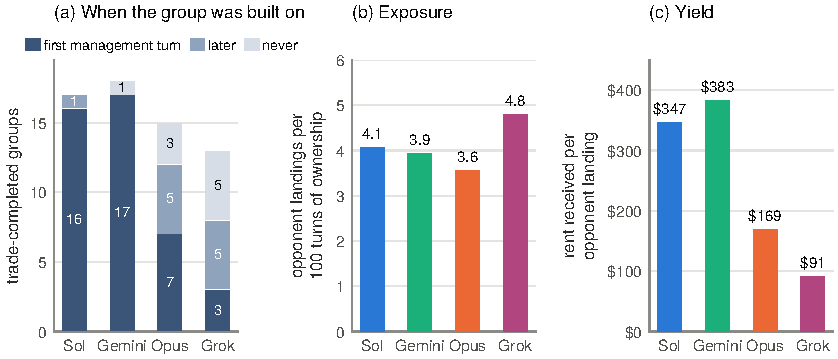
\includegraphics[width=\linewidth]{fig_conversion.pdf}
\caption{What followed a completion by trade. (a)~When the owner first built on the group. (b)~How often opponents landed on it. (c)~How much rent each landing paid. Exposure is similar across systems and the rent per landing is not.}
\label{fig:conversion}
\end{figure}

The difference in rent does not come from exposure (Figure~\ref{fig:conversion}). Opponents landed on these groups at similar rates, between \fact{d.conv.landrate.min} and \fact{d.conv.landrate.max} times per 100 turns of ownership, and Grok's groups were landed on most often. Groups built in the first management turn and groups not built then were held for similar lengths of time, with median durations of \fact{conv.trade-groups.first-window-built.median-duration} and \fact{conv.trade-groups.first-window-not-built.median-duration} turns and landing rates of \fact{d.conv.early.landrate} and \fact{d.conv.late.landrate} per 100 turns. What differs is the rent charged at each landing. Sol and Gemini received \$\fact{d.conv.rpl.Sol} and \$\fact{d.conv.rpl.Gemini} per opponent landing, Opus \$\fact{d.conv.rpl.Opus} and Grok \$\fact{d.conv.rpl.Grok}. Sol and Gemini together exceed Opus and Grok together in each of the \fact{d.conv.blocks.ordered} seed blocks. The \fact{conv.trade-groups.first-window-built.groups} groups built at once collected \$\fact{conv.trade-groups.first-window-built.rent} of the \$\fact{conv.trade-groups.total-rent} paid on all \fact{groups.routes.trade}, or \$\fact{d.conv.early.rentperlanding} per landing against \$\fact{d.conv.late.rentperlanding}. Landings are few. Five groups account for \fact{d.conv.top5.pct}\% of the rent, so the dollar totals rest on a small number of dice outcomes. Figure~\ref{fig:timeline} in the appendix draws every group.

An earlier classification, which we inherit, says why \fact{d.conv.unbuilt.n} groups went unbuilt in the first management turn. In \fact{conv.trade-groups.inherited-first-window-causes.never-legal-in-window} no build on the group was legal during that turn, and \fact{d.conv.noopt.mortgaged} of those groups held a mortgaged deed at completion. In \fact{d.conv.defaults} the engine applied a default after an invalid build request, in \fact{conv.trade-groups.inherited-first-window-causes.received-conflict} Grok's applied call ended the turn while its text requested a build, and in \fact{conv.trade-groups.inherited-first-window-causes.valid-end} the owner validly ended the turn. Opus's \fact{d.conv.unbuilt.n.Opus} unbuilt groups are \fact{inh.window.Opus.never-legal-in-window} windows with no legal build and \fact{inh.window.Opus.default-after-refusal} defaults. Part of its gap is therefore its response condition, since an invalid action-only build plan gets no correction, and part is the state in which it bought. It completed \fact{conv.trade-groups.by-model.Opus.mortgaged-deed-at-completion} of its \fact{conv.trade-groups.by-model.Opus.groups} groups with a mortgaged deed in them and held a median of \$\fact{conv.trade-groups.by-model.Opus.median-cash-after-completion} afterwards. Grok's \fact{d.conv.unbuilt.n.Grok} are \fact{inh.window.Grok.never-legal-in-window} windows with no legal build, in which its notes defer redemption to keep cash, \fact{inh.window.Grok.received-conflict} conflicting calls and \fact{inh.window.Grok.valid-end} stated holds. Grok held a median of \$\fact{conv.trade-groups.by-model.Grok.median-cash-after-completion} after its trades, enough for a house in most groups.

\IncidentTitle{g20}{Rivals try to stop a sale from becoming houses (G20)}

At G20 turn 22 Opus sells Illinois to Grok for \$500. The sale completes Grok's reds and leaves it \$222, and a red house costs \$150. Two turns later Sol's private note says \InlineQuote{in-g20-d95-cashstarved}. Gemini then says the same in public.
\TranscriptQuote{g20-d96-appeal}
Grok's next note registers the appeal.
\TranscriptQuote{g20-d97-recognition}
On its next turn Grok builds one house on each red, which leaves it \$7, and mortgages New York Avenue. It then tries to sell Vermont to Gemini.
\TranscriptQuote{g20-d100-sale}
\TranscriptQuote{g20-d101-refusal}
\IncidentOutcome{Grok mortgages Vermont for \$50. Opus later bids for two of Grok's mortgaged deeds, telling it \InlineQuote{in-g20-d129-houses}, and Grok holds out for more than Opus will pay. Opponents land on Grok's reds twice and pay \$126. Grok is the first player eliminated, at turn 84. Gemini wins.}
\IncidentReading{Gemini and Sol both treat cash paid to Grok as houses on the reds, which is the conversion this section describes, seen by the players it threatens. Gemini asks the table to withhold the cash and then refuses a purchase itself. Opus does the opposite and offers Grok money for houses. The appeal is one player's request and its own follow-through. It is not a cartel.}
\IncidentSource{G20 d95--d102, d129--d130 and d156--d160. Grok's quoted note belongs to the selected second attempt at d97, after a malformed first attempt. Opus's later bids are action-only responses.}
